\chapter{引言}
\label{cha:intro}

\section{研究意义}
\label{sec:first}
视觉是人类感知世界最直接和重要的方法之一,光线通过眼睛、视网膜、大脑等器官的处理,最终形成我们所感知的图像。随着科技的发展,数码相机、摄像机的出现使得数字图像和视频成为了人们日常生活中最常见的媒介。特别是随着近年来智能手机,移动互联网、社交网络的飞速发展和普及,人们随时随地都可以将眼前所见拍摄成图像或视频,并通过网络分享给自己在世界各地的亲朋好友。这些海量的数字图像和视频信息的处理已经成为计算机科学等领域主要的研究内容。图像和视频处理已经从基于像素的处理,例如图像去噪、图像增强、图像压缩等,逐步转移到基于内容的处理,例如基于内容的编辑、基于内容的检索等~\cite{CMM12THU}。根据经验,我们在观察图像或视频时,一般会将注意力集中在某些感兴趣区域,例如,在观看新闻联播时我们的注意力主要集中在播音员身上。生物学家和心理学家通过研究和实验证实,人类的视觉系统只对图像的某些局部进行处理,而对其余部分几乎完全忽略~\cite{treisman1980a}~\cite{Koch1985Shifts}。一般将人类视觉系统感兴趣的这类对象称为前景对象或显著性对象,相反,图像中的另外一部分则称为背景。背景减除,或前景检测,是指在图像中将前景对象和背景对象分离的一种技术。例如,在图~\ref{fig:1}中,~\ref{fig:subfig1}中为输入图像,~\ref{fig:subfig2}中为背景减除技术提取的前景对象,其中用白色表示前景区域,黑色表示背景区域。\par
\begin{figure}[h]
  \centering%
  \subcaptionbox{输入图像\label{fig:subfig1}}[3cm] %标题的长度,超过则会换行,如下一个小图。
    {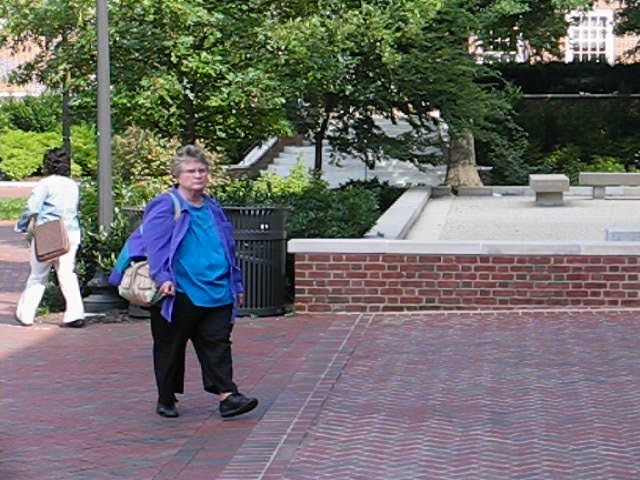
\includegraphics[height=3cm]{p2.jpg}}%
  \hspace{4em}%
  \subcaptionbox{背景减除结果,白色为前景,黑色为背景\label{fig:subfig2}}
      {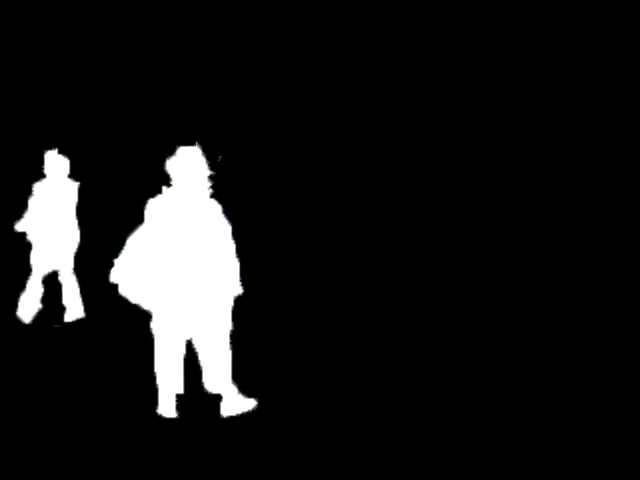
\includegraphics[height=3cm]{gtp2.png}}
  \caption{背景减除示例}
  \label{fig:1}
\end{figure}
在视频中,一般将运动的对象视为前景,相反静止的部分则归为背景。视频由连续的图像序列组成,当拍摄视频的摄像机保持固定时,分离前景和背景只需考察对象的运动。而当
拍摄视频的摄像机也存在旋转、平移、缩放等运动时,造成视频中所有像素都产生运动。这时,可以通过区分相机引起的运动和前景产生的运动来区分前景和背景。
作为计算机尝试分析并理解图像的第一步,背景减除是图像处理、视频监控、目标识别与跟踪、基于深度的绘制(Depth Image Based Rendering,DIBR)等应用领域中重要的预处理步骤。例如,在内容感知的图像缩放应用中,为了在对图像进行缩放编辑时保持前景对象的比例,首先需要对图像进行显著性分析,确定显著性对象的位置。在DIBR中,为了处理因遮挡而产生的空洞,需要利用图像中的其它像素对空洞进行填充。因为被遮挡的部分基本上是背景区域,因此如果误将前景像素填充到空洞中,会造成鬼影、闪烁等问题,影响绘制视频的质量。利用背景减除技术对视频进行预处理,可以有效避免将前景像素用于空洞填充,提高视频的绘制质量。人类的视觉系统与生俱来具有这种能力,然而在计算机上实现视频图像中的背景减除却十分困难。主要的困难在于:
 \begin{itemize}
    \item 噪声干扰。在环境噪声的干扰下,我们得到的图像中可能包含一些噪声,这些噪声会对前景提取的准确度造成重要的影响。例如
    在雨雪天气或者夜间拍摄的图像中,存在亮度不足,雨雪对前景判别产生干扰等问题;
    \item 前景的多样性和不确定性。在不同的场景下,前景对象的定义存在不确定性,例如,在一张汽车广告画中汽车是前景对象,然而同样是汽车,
    在车模的特写照片中却成为背景。
    \item 动态背景,在视频背景减除中,我们在判别前景和背景时一般假设背景区域的像素是静止,而运动的像素
    则属于前景。然而,在实际应用中,这一假设并不总是成立。例如视频中被风吹动摇摆的树叶,喷泉,以及流动的水面等。这些对象虽然是运动
    的,但实际却属于背景;
    \item 相机的运动,在早期的视频背景减除技术研究中,一般假设相机是静止的。然而,随着移动计算平台,例如手机、手持摄像机、智能机器人等,
    的出现,移动相机拍摄视频中的背景减除技术研究越来越重要。在移动相机拍摄的视频中,区分相机运动和前景运动是一项困难的工作。
  \end{itemize}

\par
综上所述,背景减除技术是计算机视觉研究中一个非常热门的课题。提高背景减除技术的准确度和速度对于众多
应用具有十分重要的意义。
\section{相关工作概述}
\label{sec:second}

\subsection{静止相机情况下的视频背景减除}
\label{sec:staticCamera}
在早期的视频背景减除技术研究中,一般假设摄像机是静止的。基于这一假设,通过建立不包含前景对象的背景模型,并将其它图像帧与背景模型进行比较得到前景。
在图~\ref{fig:2}中是一个典型的视频背景减除算法流程图。假设输入视频帧的前$N$帧图像中不包含前景对象,利用这些图像初始化背景模型,在$t$时刻得到的背景模型为$B(t)$。
在下一时刻,将视频图像帧$I(t)$与$B(t)$进行匹配,其中匹配成功的像素标记为背景,反之则为前景。最后利用所得前景结果和当前帧信息对$B(t)$进行更新,得到$B(t+1)$。
由此可见,背景模型的对算法的准确度至关重要。

\begin{figure}[h]
  \centering%
  {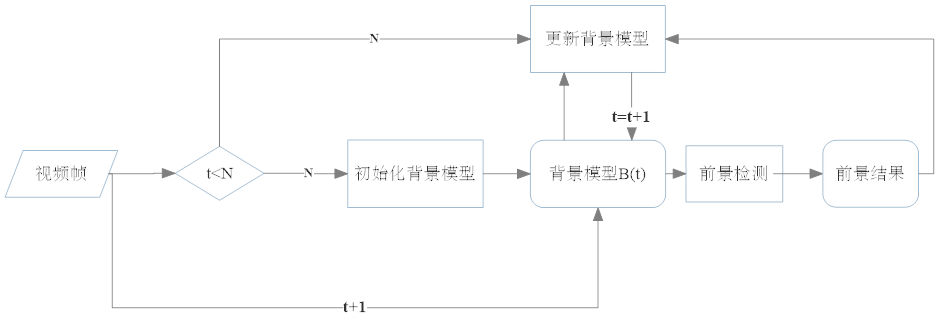
\includegraphics[width=0.85\textwidth]{bsflowchart.png}}%
  \caption{背景减除流程图~\cite{BouwmansOverview}}
  \label{fig:2}
\end{figure}
最简单的背景模型可以通过对输入视频帧进行平均~\cite{LeeAverage}或者中值滤波~\cite{MF}的方式得到,然而这种方法对噪声的处理并不理想。为了解决这一问题,研究人员提出了一系列基于统计模型的背景建模方法。Chien等人~\cite{Chien2002Efficient}提出了一种基于图像注册背景建模方法,利用一幅图像作为背景模型。该方法首先对视频相邻帧进行
差分操作,并对结果进行二值化得到掩码图像$M$。$M$中值为0的像素为相邻帧图像亮度变化在门限之内的像素,这些像素属于背景的概率较大;然后,观察连续多帧图像产生的$M$,若$M$中某像素长期为0,则其被判为可靠背景像素,并将当期图像帧此位置的像素值复制到背景图像中;最后,将后续的视频帧与背景图像进行差分操作得到前景结果,并对背景图像进行更新。该方法
简单高效,但其依赖固定门限,且仅以一幅图像作为背景模型,无法处理亮度变化大以及包含动态背景的视频。假设视频中像素的亮度值的变化可以用高斯模型来建模,Wren等人~\cite{Wren}提出了单高斯背景模型,随后Kim等人~\cite{kim2007robust}对其进行了改进。然而,这种单高斯模型无法处理像被风吹动的树叶、流动的水等这种动态背景。Stauffer~\cite{stauffer1999adaptive}等人提出了基于自适应混合高斯模型的背景模型建模方法,利用多个高斯模型对背景像素进行建模。相比于单高斯模型,混合高斯模型处理亮度变化大及包含动态背景的视频时效果虽然得到了显著提升,但其前景误检率仍较高。Barnich等人~ \cite{Barnich2011ViBe}提出了一种名为ViBe的无参数采样模型背景建模方法。该方法通过$N$个背景图像色彩空间采样值来描述背景模型:
$$M(x)=\{v_{1},v_{2},...,v_{N}\}$$ \par
如图~\ref{fig:vibe}所示,为了区分某像素$v(x)$是否属于背景,ViBe算法在二维欧几里德色彩空间内计算以$v(x)$为中心的圆形范围$S_{R}(v(x))$内的采样值与背景模型$M(x)$交集的数量,当$\#\{S_{R}(v(x))\bigcap\{v_{1},v_{2},...,v_{N}\} \}$大于或等于某门限值时像素$v(x)$被判为背景,否则为前景。

\begin{figure}[h]
  \centering%
  {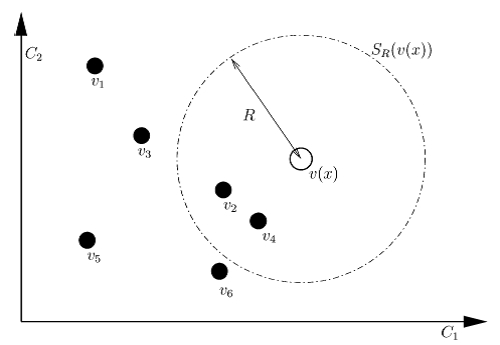
\includegraphics[width=0.5\textwidth]{vibe.png}}%
  \caption{ViBe算法示意图~\cite{Barnich2011ViBe}}
  \label{fig:vibe}
\end{figure} \par


在背景模型初始化过程中,ViBe算法在第一帧图像中按照均匀分布随机的从像素邻域中选取像素值:${M}^{0}(x)=\{v^{0}(y\mid y\in N_{G}(x))\}$。虽然这种初始化方法可能会将在第一帧中的移动对象设为背景从而产生鬼影现象,但是随着模型的更新,这种现象会逐渐消失。ViBe算法使用一种新的保守的背景更新策略,与之前的更新方法不同的是该算法从背景像素点的历史值中收集样本值,不断更新随机时间序列,当新的样本值加入到背景模型中时随机地将历史样本值丢弃。具体的说,ViBe定义背景模型中的采样值在更新时保留的概率为:
$$P(t,t+dt)={\left(\frac{N-1}{N} \right)}^{(t+dt)-t}$$ \par
另外,为了降低背景更新的频率,ViBe算法还采用时间采样的方式来延长模型的生命周期。若某像素被分类为背景,则以一定的概率(如$\frac{1}{16}$)用该像素的值去更新模型。为了保证空间一致性并使被前景区域覆盖的背景点被更新,在更新时将当前帧$x$点处的像素值去更新在空间八邻域上的邻近像素点的背景模型。ViBe算法简单,鲁棒性强,但也存在一些缺陷:
 \begin{itemize}
\item 当运动目标与背景对比度小的情况下,ViBe 算法提取的目标轮廓存在缺陷,导致目标轮廓不封闭,容易产生轮廓内部孔洞现象;
\item 监控场景下的运动目标有阴影时算法检测出的前景存在阴影现象。
\end{itemize}
\par
Droogenbroeck等人对ViBe算法进行了改进~\cite{vibe},主要修改了距离函数和判别门限,区分更新蒙版和输出蒙版并对其进行了滤波,在更新背景模型时对某些像素进行了限制,当视频中摄像机有抖动时,增大更新系数并检查像素的闪烁。修改后的ViBe算法比原算法普适性更强,并且在检测正确率等方面也有所提高。Hofmann等人~\cite{pbas}提出了一种带反馈的基于像素的自适应视频背景分割算法, 称为PBAS。该方法和ViBe算法一样都是无参数方法。该方法的基本思想和ViBe类似,主要的区别在于PBAS通过自适应的方法对模型更新相关参数进行自适应调整。这种自适应调整通过闭环反馈的方式实现,背景判决门限和更新率等参数可以在处理过程中通过反馈的方式自适应调整,调整后的参数可以获得更好的性能。在测试中PBAS方法的检测准确率等性能参数超过了ViBe,而且同样可以实现实时检测。在近期的一项工作中 \cite{subsenseTIP}, 作者提出了一种更加有效的反馈式模型更新背景建模方法,SuBSENSE. 该算法的准确度在CD.Net 2012 和CD.Net 2014数据集中均优于其它算法。因为同样是基于采样模型,该算法效率高且易于实现。\par
与上述算法不同,Lin等人~\cite{lin2002a}引入了更复杂的统计模型支持向量机模型(Support Vector Machine,SVM),利用SVM分类器对所有训练视频帧像素进行分类并添加到背景模型,直到不出现新的背景像素时停止模型初始化。SVM所用的特征包括光临信息和图像帧间的差分图像。此外,研究人员还提出了基于子空间学习~\cite{uray2007incremental}和基于频域分析~\cite{Gao2009}的背景模型。文献~\cite{BouwmansOverview}对这些算法进行了总结和分类。

\subsection{移动相机情况下的视频背景减除}
\label{sec:movingCamera}
随着移动计算平台(如智能手机、手持摄像机、智能机器人等)的快速发展, 移动相机视频越来越普及, 针对移动相机拍摄视频的背景减除技术越来越重要。 与静止相机的情况相比, 移动相机下的背景减除要困难很多, 因为相机的运动使得视频中前景和背景像素都会产生运动, 区分相机产生的运动和前景自身运动是待解决的主要难题。另外,如果能利用图像帧准确估算出相机运动,并进行运动补偿,就可以将移动相机情况转换为固定相机情况处理。
 文献~\cite{iccv2009}提出一种基于点轨迹的背景减除算法, 根据背景点轨迹矩阵的秩等于3的特点~\cite{Tomasi_1992}, 以滑动窗口的方式利用随机抽样一致(random sample consensus, RANSAC)算法~\cite{Ransac}在点轨迹矩阵中检测背景点。 同样基于点轨迹并考虑前景像素的集中性, 文献~\cite{Cui2012}提出一种基于点轨迹矩阵分解的算法。Berger等~\cite{SubspaceTracking}提出一种基于线性子空间跟踪的背景建模算法, 与基于点轨迹的同类算法相比, 该算法的背景检测更准确, 且处理速度更快, 但其处理一帧图像仍需要1.6s。 另外, 由于这类算法是基于点轨迹的, 而计算视频中稠密像素的长期轨迹是一项十分耗时且困难的工作, 即使在GPU加速的情况下也需要几秒的时间处理一帧图像~\cite{ECCV10DensePonintTrajectories}。\par

为了处理相机的运动, 另一类算法引入了稠密光流。 文献~\cite{kwak2011Generalized}提出一种基于贝叶斯滤波的背景减除算法框架, 该算法需要视频第一帧的准确前景作为输入, 并在随后的视频帧中利用稠密光流信息进行可靠跟踪; 这种算法需要人工交互来生成第一帧的准确前景, 不适用于在线处理, 且无法处理长时间且包含复杂相机运动的视频. 文献~\cite{gbsuperpixel}提出另外一种基于稠密光流的移动相机视频背景减除新算法, 通过建立基于超像素的背景模型, 并基于二进制置信传播技术通过多次迭代获得像素级精度的前景; 虽然该算法的准确度要优于其他算法, 但其处理一帧大小为300×200的视频帧需要6s。\par
文献~\cite{5.8s}提出一种实时的移动相机下视频背景减除算法, 该算法利用基于固定特征点跟踪的相机运动估算算法和简化的双模高斯背景模型, 速度较快, 可以实现实时处理; 但没有给出该算法前景检测准确度的定量分析。 本文通过实验发现, 文献~\cite{5.8s}算法的前景检测准确度较低, 特别是在相机移动幅度较大的情况下, 无法适应前景检测准确率要求较高的应用。\par
一般采用单应性矩阵或基础矩阵来来描述相机运动情况。 文献.~\citenum{Multitransform}中提出了一种多变换模型的方法来处理相机运动。该算法根据相邻帧图像的几何变换情况,自适应的从单应性矩阵模型和基础矩阵模型中选择一个模型。当选择单应性矩阵时,根据特征点的运动情况估算全局单应性基础并用于相机运动补偿,而当选择矩阵模型使用时,基于最小均方误差的方式在一系列单应性矩阵中选择一个误差最小的单应性矩阵作为全局参数补偿相机运动。\par
国内研究人员方面,崔智高等~\cite{czg}提出一种基于多组单应约束和马尔可夫随机场的移动目标检测算法, 通过轨迹分离和像素标记2个阶段实现移动相机拍摄视频中运动目标的检测; 该算法检测前景的准确度较高, 但由于算法是基于点轨迹的, 同样存在算法计算量大无法实现实时处理的问题。

\subsection{图像显著性分析}
\label{sec:imageSaliency}
图像显著性区域检测的目标是在计算机上实现像人眼一样快速判断图像中显著性区域的能力,通过这种技术提取的图像显著性区域可以广泛用于目标识别,图像编辑以及图像检索等应用。Itti等人~\cite{itti}提出了最早的显著性检测模型,该模型结合了认知心理学,神经科学和计算机科学的理论和方法。基于人类注意力自底向上,关注中心与四周差异的特点,该模型预测人眼观察图像时的焦点,能得到一系列离散的圆点形状的显著性区域预测结果,并不能得到显著性对象的准确边界。随后,显著性检测研究的热点集中在如何获得显著性对象的准确边界,并把它们从图像中分割出来。在这种情况下,显著性检测可以被看作是一个图形分割问题,目标是把图形分割为显著的和非显著的两个部分。\par
最近几年年以来,显著性区域检测问题一直是计算机视觉等相关研究领域的研究热点~\cite{saliencySurvey}。研究人员提出了一系列新算法,这些算法使得显著性对象的准确度不断提高,算法的速度也有了显著提高。一般认为,在定位显著性对象时一般依靠内部和外部两种线索\cite{saliencySurvey},其中内部线索来自于待处理图像自身,而外部线索可能来自于用户交互或来自于其它图像的信息。从应用和效率的角度来说,基于内部线索的算法更加贴近实际应用。早期,研究人员关注的内部线索主要是显著性对象的独特性(Uniqueness)。

\subsection{图像填充技术}
\label{sec:imageInpainting}

\section{论文研究内容}
\label{sec:contents}


\section{本文的组织结构}
\label{sec:hierarchy} 